\sloppy
\documentclass[14pt,a4paper,oneside]{extarticle}	% Размер основного шрифта и формата листа
\usepackage{xltxtra}						% Используется для вывода логотипа XeLaTeX
\usepackage{xunicode}						% Кодировка документа
\usepackage{polyglossia}					% Загружает пакет многоязыковой верстки
\newfontfamily\russianfont{Book Antiqua}
%\setmainfont{Liberation Serif}						% Основной шрифт текста
\setmainfont{Book Antiqua}
\setdefaultlanguage{russian}				% Основной язык текста
\setotherlanguage{english}					% Дополнительный язык текста
\linespread{1}							% Межстрочный интервал выбран полуторным
\usepackage[left=2.5cm,
right=1.5cm,vmargin=2.5cm]{geometry} % Отступы по краям листа
\bibliographystyle{ugost2008}

\usepackage{xcolor}
\usepackage{hyperref}
% Цвета для гиперссылок
\definecolor{linkcolor}{HTML}{359B08} % цвет ссылок
\definecolor{urlcolor}{HTML}{799B03} % цвет гиперссылок
\hypersetup{pdfstartview=FitH,  linkcolor=linkcolor,urlcolor=urlcolor, colorlinks=true}

%---------------------------%
%---- Пакеты расширений ----%
%---------------------------%
\usepackage{xcolor}
\usepackage{hyperref}
% Цвета для гиперссылок
\definecolor{linkcolor}{HTML}{359B08} % цвет ссылок
\definecolor{urlcolor}{HTML}{799B03} % цвет гиперссылок
\hypersetup{pdfstartview=FitH,  linkcolor=linkcolor,urlcolor=urlcolor, colorlinks=true}


\usepackage{verbatim,indentfirst}
\usepackage{cite,enumerate,float}
\usepackage{amsmath,amssymb,amsthm,amsfonts}

%---------------------------%
%--- Вставка иллюстраций ---%
%---------------------------%
\usepackage{graphicx}
\usepackage{subfigure}
\usepackage{fontspec}
%\graphicspath{{Images/}}

\begin{document}
%\pagestyle{empty} %  выключаенм нумерацию
%\setcounter{page}{3}% Нумерация начинается с третьей страницы
%\renewcommand{\contentsname}{\center{Содержание}}
%\tableofcontents

\begin{center}
	\section*{Выдергивание листа бумаги из-под стакана}
\end{center}

\begin{figure}[H] 	
	\centering 	
	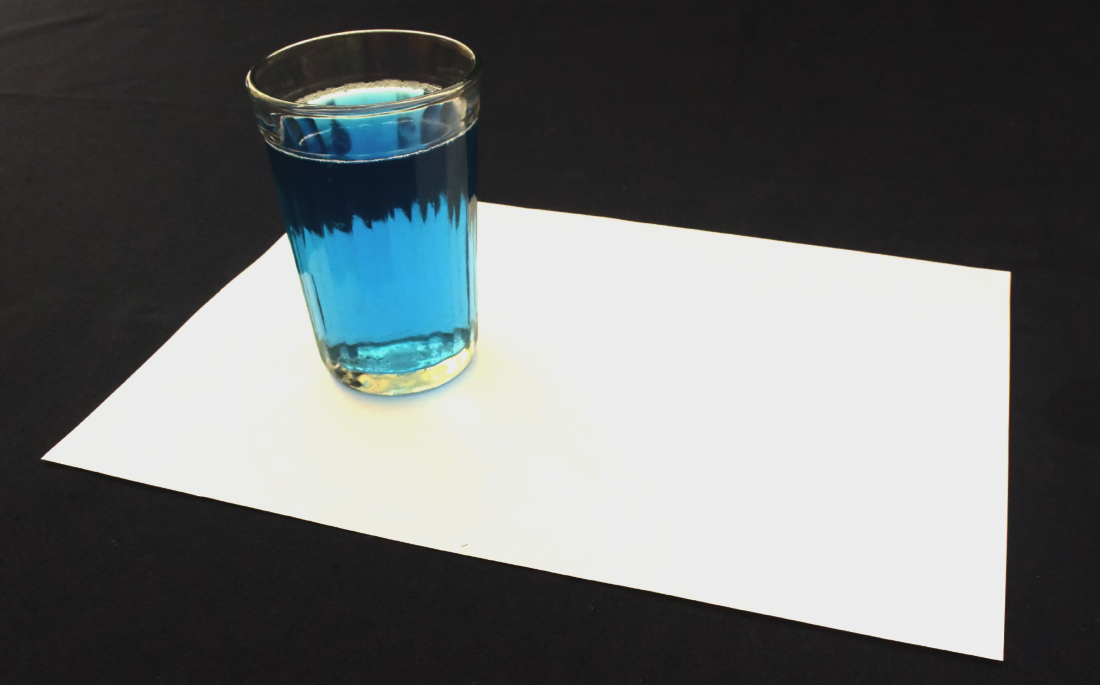
\includegraphics[width=0.9\linewidth]{inertia-1.png}
	\caption{Демонстрация явления инертности}
\end{figure}

\subsection*{\underline{Оборудование:}}

\begin{enumerate}
\item Лабораторный стол с гладкой поверхностью.
\item Стакан с водой.
\item Лист бумаги.
\end{enumerate}

\newpage
\subsection*{\underline{Основные понятия:}}

Инерция, инертность (в механике) — свойство материальных тел, «сопротивляться» воздействию силы.
Многочисленные опыты позволили Г. Галилею (1564–1642) впервые сформулировать свой знаменитый закон инерции:

\begin{flushleft}
	
	\textit{тела, свободные от внешних воздействий (сил), сохраняют состояние 
покоя или равномерного прямолинейного движения относительно 
Земли}
\end{flushleft}


Впоследствии английский физик И. Ньютон (1643–1727) включил этот закон в число общих законов движения, поэтому закон инерции часто называют первым законом Ньютона. 
Все системы отсчета, для которых выполняется первый закон 
Ньютона, получили название инерциальных систем. 

Когда внешние воздействия на тело (силы) отсутствуют или взаимно уравновешиваются, инертность проявляется в том, что тело сохраняет неизменным состояние своего движения или покоя по отношению к инерциальной системе отсчета.
Если же на тело действует неуравновешенная система сил, то свойство инертности сказывается в том, что изменение состояния покоя или движения тела, т. е. изменение скоростей его точек, происходит постепенно, а не мгновенно; при этом движение изменяется тем медленнее, чем больше инертность тела.
Величина, количественно определяющая инертные свойства 
тела, называется массой тела. 

\newpage
\subsection*{\underline{Краткое описание демонстрации:}}

Для демонстрации инертности тел стакан с водой располагают на ровной горизонтальной поверхности.
Под стаканом помещают обычный лист бумаги.
Если начать тянуть лист с такой силой, чтобы он не проскальзывал относительно стакана, то стакан станет двигаться вместе с бумагой.
В этом случае сила трения, приложенная к стакану со стороны бумаги, действует длительное время и сообщает ему  необходимое количество движения (импульс), чтобы стакан перемещался вместе с бумагой. 

Если же бумажный лист резко с большой силой выдернуть, то он выскользнет из-под стакана, 
а сам стакан останется стоять на месте. 
Теперь время действия силы трения на стакан мало, причем оно равно времени прохождения конца 
бумажного листа под дном стакана.
За это время сила трения успевает сообщить стакану очень малый импульс, и стакан остается 
на месте. 

\newpage
\subsection*{\underline{Теория:}}

Используя второй закон Ньютона в проекции на горизонтальную ось $ x $, имеем:
\begin{equation}\label{inertia-eq1}
\frac{\partial p_{x}}{\partial t} = F_{x},
\end{equation}
где $ p_{x}=mv_{x} $ — проекция импульса на ось \textit{x}.
Так как проекция скорости $v_{x}$ является производной координаты \textit{x} по времени, получается следующее:
 
 \begin{equation}\label{inertia-eq2}
 m\frac{d^{2} x}{d t^{2}} = F_{x}.
 \end{equation}

При проскальзывании на стакан со стороны листа бумаги действует постоянная сила трения скольжения, равная $ F_{x} = \mu mg $ (где через $\mu$ обозначен коэффициент трения между стаканом и листом). В этом случае стакан будет двигаться с постоянным ускорением $a = \mu g$ и за время выдергивания листа бумаги переместится на расстояние:
\begin{equation}\label{inertia-eq5}
\Delta x = \mu g\Delta t^{2}/2.
\end{equation}

Из уравнения (\ref{inertia-eq5}) видно, что чем меньше время действия силы \textit{F} на лист бумаги, тем меньше перемещение $ \Delta x $ стакана.
Поэтому в пределе \mbox{$ t\longrightarrow0 $} стакан остается неподвижным относительно поверхности стола.  

\end{document}